%%%%%%%%%%%%%%%%%%%%%%%%%%%%%%%%%
%% Información para la portada %%
%%%%%%%%%%%%%%%%%%%%%%%%%%%%%%%%%

\newcommand{\AutoresEmails}{%
	Benasco Sánchez, Damián & \texttt{d.benasco@alumnos.upm.es} \\
	Sánchez Carmona, Germán & \texttt{german.sanchez.carmona@alumnos.upm.es} \\
	Vega Ortiz, Jorge Enrique & \texttt{jorge.vega@alumnos.upm.es} \\
}

\newcommand{\Asignatura}{ Inteligencia Artificial Explicable }

\newcommand{\TituloProyecto}{ Predicción de la dificultad de pago\\ mediante modelos explicables }

\newcommand{\SubtituloProyecto}{ Proyecto de la Unidad 2 · Fase II }

\newcommand{\Profesor}{ }

\newcommand{\Departamento}{ MÁSTER EN INTELIGENCIA ARTIFICIAL }

\newcommand{\Fecha}{13 de octubre de 2026}

% -*-coding: utf-8 -*-
% !TEX root = ../report.tex
\documentclass[a4paper,11pt,openany]{book}
\usepackage[utf8]{inputenc}
\usepackage[T1]{fontenc}
\usepackage[english,spanish,es-lcroman]{babel}
\usepackage{bookman}
\decimalpoint
\usepackage{graphicx}
\usepackage{amsfonts,amsgen,amsmath,amssymb}
\usepackage[top=3cm, bottom=3cm, right=2.54cm, left=2.54cm]{geometry}
\usepackage{afterpage}
\usepackage{colortbl,longtable}
\usepackage[
  pdftex,
  pdftitle={Proyecto de Inteligencia Artificial Explicable},
  pdfborder={0 0 0}
]{hyperref}
\usepackage{pdfpages}
\usepackage{url}
% Permite dividir identificadores largos en los márgenes de línea.
\let\texttt\path
\usepackage[stable]{footmisc}
\usepackage{parskip} % para separar párrafos con espacio.

% Ajuste del espaciado vertical: parskip por defecto se estira y deja
% huecos grandes en páginas con figuras, así que se fija y se reduce el
% espacio alrededor de los flotantes.
\setlength{\parskip}{5pt}%
\setlength{\intextsep}{7pt}%
\setlength{\textfloatsep}{9pt}%
\setlength{\floatsep}{9pt}%

\usepackage{lscape}
\usepackage{pgfgantt}



\usepackage{float}
\usepackage{flafter} % evita que un flotante aparezca antes de su referencia
\usepackage{subfigure}

%%-----------------------------------------------
\usepackage{fancyhdr}
\pagestyle{fancy}
\fancyhf{}
\fancyhead[LO]{\rightmark}
\fancyhead[RE]{\rightmark}
\setlength{\headheight}{1.5\headheight}
\cfoot{\thepage}

\addto\captionsspanish{ \renewcommand{\contentsname}
  {Índice general} }
\setcounter{tocdepth}{4}
\setcounter{secnumdepth}{4}

\renewcommand{\chaptermark}[1]{\markboth{\textbf{#1}}{}}
\renewcommand{\sectionmark}[1]{\markright{\textbf{\thesection. #1}}}
\newcommand{\HRule}{\rule{\linewidth}{0.5mm}}
\newcommand{\bigrule}{\titlerule[0.5mm]}

\usepackage{appendix}
\renewcommand{\appendixname}{Anexos}
\renewcommand{\appendixtocname}{Anexos}
\renewcommand{\appendixpagename}{}
\usepackage{dcolumn}
\newcolumntype{.}{D{.}{\esperiod}{-1}}
\makeatletter
\renewcommand{\@makechapterhead}[1]{%
  \vspace*{20\p@}%
  {\parindent \z@ \raggedright \normalfont
    \ifnum \c@secnumdepth >\m@ne
      \if@mainmatter
        \huge\bfseries \@chapapp\space \thechapter
        \par\nobreak
        \vskip 20\p@
      \fi
    \fi
    \interlinepenalty\@M
    \Huge \bfseries #1\par\nobreak
    \vskip 40\p@
  }}
\renewcommand{\@makeschapterhead}[1]{%
  \vspace*{20\p@}%
  {\parindent \z@ \raggedright
    \normalfont
    \interlinepenalty\@M
    \Huge \bfseries #1\par\nobreak
    \vskip 40\p@
  }}
\addto\shorthandsspanish{\let\esperiod\es@period@code}
\makeatother
%%-----------------------------------------------
%% Estilos código de lenguajes: Consola, C, C++ y Python
%%-----------------------------------------------
\usepackage{color}

\definecolor{gray97}{gray}{.97}
\definecolor{gray75}{gray}{.75}
\definecolor{gray45}{gray}{.45}

\usepackage{listings}
\lstset{ frame=Ltb,
  framerule=0pt,
  aboveskip=0.5cm,
  framextopmargin=3pt,
  framexbottommargin=3pt,
  framexleftmargin=0.4cm,
  framesep=0pt,
  rulesep=.0pt,
  backgroundcolor=\color{gray97},
  rulesepcolor=\color{black},
  %
  stringstyle=\ttfamily,
  showstringspaces = false,
  basicstyle=\scriptsize\ttfamily,
  commentstyle=\color{gray45},
  keywordstyle=\bfseries,
  %
  numbers=left,
  numbersep=6pt,
  numberstyle=\tiny,
  numberfirstline = false,
  breaklines=true,
}

% Puedes añadir más lenguajes siguiendo un estilo similar al de Python,
% o hacerte tu propio estilo.
% Enlace con alguna ayudita: www.overleaf.com/learn/latex/Code_listing
\lstnewenvironment{listing}[1][]
                  {\lstset{#1}\pagebreak[0]}{\pagebreak[0]}
                    \lstdefinestyle{consola}{
                                    basicstyle=\scriptsize\bf\ttfamily,
                                    backgroundcolor=\color{gray97}}
                    \lstdefinestyle{C}{
                                    basicstyle=\scriptsize,
                                    frame=single,
                                    language=C,
                                    numbers=left}
                    \lstdefinestyle{C++}{
                                    basicstyle=\small,
                                    frame=single,
                                    backgroundcolor=\color{gray75},
                                    language=C++,
                                    numbers=left}
                    \lstdefinestyle{Python}{
                                    basicstyle=\small,
                                    frame=single,
                                    backgroundcolor=\color{gray75},
                                    language=Python,
                                    numbers=left}


\usepackage{booktabs}
\usepackage{tabularx}
\usepackage{makecell}
\usepackage{caption}
\usepackage{enumitem}
\usepackage{microtype}

\geometry{top=2.5cm,bottom=2.5cm,left=2.4cm,right=2.4cm}
\setlength{\parskip}{3pt}
\setlength{\intextsep}{7pt}
\setlength{\textfloatsep}{9pt}
\setlength{\floatsep}{9pt}

\DeclareRobustCommand{\var}[1]{\path{#1}}

\renewcommand{\thesection}{\arabic{section}}
\renewcommand{\thesubsection}{\thesection.\arabic{subsection}}
\renewcommand{\thesubsubsection}{\thesubsection.\arabic{subsubsection}}

\addto\captionsspanish{%
  \renewcommand{\tablename}{Tabla}%
  \renewcommand{\figurename}{Figura}%
}

\begin{document}
\raggedbottom 
\begin{titlepage}

  \begin{minipage}{0.16\linewidth}
    \hspace*{0.3cm}
    \noindent
    
\includegraphics[width=\linewidth]{./include/EscUpm.png}
  \end{minipage}\hfill
  \begin{minipage}{0.68\linewidth}
    \begin{center}
      \huge{ Universidad Politécnica\\de Madrid }\\
      \vspace*{0.5cm}
      \Large{\textbf{Escuela Técnica Superior de Ingenieros Informáticos}}\\
      \vspace*{0.3cm}
      \Large{\textbf{Máster en Inteligencia Artificial}}
    \end{center}
  \end{minipage}\hfill
  \begin{minipage}{0.16\linewidth}
    
\includegraphics[width=\linewidth]{./include/FacInformatica.png}
  \end{minipage}

  \vspace*{1cm}
  \begin{center}
    \Large{\Asignatura{} }
  \end{center}

  \vspace*{1cm}
  \begin{center}
    \huge\bfseries {  \TituloProyecto{} }\\[0.5cm]
    \Large{\SubtituloProyecto{}}
  \end{center}

  \vspace*{3.6cm}

  \begin{center}
    \large\textbf{Grupo 3}\\[0.2cm]
  \end{center}
  {\small
  \begin{tabular}{@{}l@{\hspace{0.6cm}}l@{}}
    \AutoresEmails
  \end{tabular}}\\[0.4cm]
  % \large{Profesor: \Profesor{} }


  \vspace*{2.8cm}
  \begin{center}
    Madrid, \Fecha
  \end{center}

\end{titlepage}


% Índice general en numeración romana (materia preliminar).
\pagenumbering{roman}
\tableofcontents
\clearpage

\pagenumbering{arabic}
\setcounter{page}{2}

\section{Introducción}\label{sec:intro}

El objetivo del proyecto es predecir si un cliente tendrá dificultades de pago el mes siguiente, variable \var{payment_difficulty_next_month}. La Fase I se limitó deliberadamente al modelo lógico, un árbol de decisión, con el fin de obtener reglas que permitieran entender qué perfiles eran asignados a cada clase. La Fase II amplía ese propósito y compara tres familias de modelos (árbol, regresión logística y modelo aditivo explicable, EBM) no solo por su capacidad de discriminación, sino por el tipo de explicaciones globales y locales que cada una hace posibles. Por tanto, el objetivo no es únicamente obtener una predicción, sino justificar el compromiso entre rendimiento y legibilidad.

El análisis se realiza sobre el conjunto de entrenamiento, que contiene 25\,000 observaciones y 15 predictores, 11 numéricos y 4 categóricos. El conjunto de test, con 5\,000 filas y sin etiquetas, se reserva para la predicción final y no interviene en el desarrollo. Los datos provienen de \emph{Default of Credit Card Clients} \cite{uci}. Dado que la clase positiva es minoritaria, con 5\,303 casos (21,21\,\%) frente a 19\,697 (78,79\,\%), la evaluación debe considerar el comportamiento en ambas clases. Predecir siempre la clase mayoritaria bastaría para alcanzar un 78,79\,\% de exactitud, una cifra que por sí sola no informa sobre la detección de dificultades de pago.

Para que la comparación sea homogénea, las tres familias se evalúan sobre las mismas cinco particiones externas, agrupadas por perfil idéntico de los quince predictores, con validación cruzada anidada dentro de cada entrenamiento. La agrupación evita que perfiles repetidos, 31 en total y 13 con etiquetas distintas, aparezcan simultáneamente en entrenamiento y validación; el anidamiento separa la selección de hiperparámetros de la estimación del rendimiento. La configuración se elige por ROC-AUC medio y el umbral por exactitud equilibrada medio. La comparación final emplea ROC-AUC, exactitud (accuracy) equilibrada, F1, sensibilidad (recall), precisión y exactitud, con la clase positiva igual a uno. El test permanece intacto hasta el ajuste del modelo final.

Los resultados muestran una jerarquía consistente entre particiones. El EBM alcanza la mayor ROC-AUC ($0{,}7755 \pm 0{,}0077$) y la mejor exactitud equilibrada con umbral interno (0,6997), seguido de la regresión logística ($0{,}7515 \pm 0{,}0075$) y del árbol ($0{,}7372 \pm 0{,}0044$). Los umbrales internos mejoran la detección de la clase positiva a costa de precisión y exactitud. Con 0,5 los tres modelos superan la referencia mayoritaria, pero detectan menos del 30\,\% de los positivos. El modelo final es un EBM sin interacciones, con \var{max_bins}=32, un mínimo de 10 observaciones por hoja y umbral 0,20. Aplicado al test, asigna 3\,208 casos a la clase 0 (64,16\,\%) y 1\,792 a la clase 1 (35,84\,\%); sin etiquetas reales no pueden calcularse métricas sobre esa salida.

El informe describe a continuación el método y el protocolo de evaluación, presenta los resultados comparados, analiza las explicaciones globales y locales de cada familia, discute sus implicaciones y límites, y cierra con las conclusiones.

\section{Método}\label{sec:method}

El entrenamiento contiene 25\,000 observaciones y 15 predictores, 11 numéricos y 4 categóricos. La variable objetivo, \var{payment_difficulty_next_month}, es binaria y la clase positiva supone el 21,21\,\%; el test reservado tiene 5\,000 filas sin etiquetas. El preprocesamiento se ajusta dentro de cada entrenamiento y se aplica a su validación, mientras que el test permanece intacto hasta la predicción final. El árbol usa one-hot sin escalado, la logística estandariza las numéricas y usa one-hot con la primera categoría como referencia, para que la penalización no dependa de la escala; y el EBM conserva los valores originales y discretiza internamente.

\subsection{Protocolo de evaluación}

Las tres familias se comparan sobre las mismas cinco particiones externas, estratificadas y agrupadas por perfil idéntico de los 15 predictores, cada registro se valida una vez. El agrupamiento es necesario porque hay 29 perfiles distintos repetidos, que aportan 31 registros adicionales; 13 de esos perfiles tienen etiquetas distintas. Si las copias se repartieran entre entrenamiento y validación, la evaluación mediría en parte la memorización del perfil. Dentro de cada entrenamiento externo se ejecutan cinco particiones internas. La configuración se elige por ROC-AUC media interna y el umbral por exactitud equilibrada media interna, con una rejilla de 0,05 a 0,95 en pasos de 0,05; los empates se resuelven hacia el valor más cercano a 0,5 y después hacia el menor.

El anidamiento evita el optimismo de elegir configuración y umbral con los mismos datos usados para informar el rendimiento; la partición externa no participa en esas decisiones. Se informan ROC-AUC, exactitud, exactitud equilibrada, sensibilidad, precisión y F1, con la clase 1 como positiva. La referencia mayoritaria siempre predice 0, con exactitud $0{,}7879 \pm 0{,}0052$, ROC-AUC y exactitud equilibrada 0,5000, y sensibilidad, precisión y F1 nulos. El umbral no se fija en 0,5 porque el desequilibrio favorece a la clase mayoritaria; la exactitud equilibrada obliga a considerar ambas clases.

\subsection{Árbol de decisión}

Se empleó un árbol CART con impureza de Gini, pues este criterio produce divisiones binarias traducibles directamente en reglas. La rejilla de búsqueda combina profundidad máxima 1, 2 y 3 con un mínimo de 50, 200 o 500 muestras por hoja, con nueve configuraciones y 255 ajustes. Esta restricción mantiene entre 2 y 8 hojas, un tamaño presentable como lista de reglas, y no impone la profundidad 2 de la Fase I, ya que la validación puede elegir 1, 2 o 3.

Un árbol sin restricciones sirvió de diagnóstico. Su ROC-AUC de entrenamiento próxima a 1, exactitud 99,95\,\%, profundidad de 37 a 54 y entre 3\,522 y 3\,673 hojas, frente a ROC-AUC de validación 0,5985. El contraste evidencia sobreajuste y justifica la restricción. No se usaron pesos de clase porque modifican la distribución efectiva y la probabilidad aprendida, mientras que el umbral ya se ajusta para el desequilibrio. Tampoco se añadió poda posterior, porque la rejilla ya controla la complejidad. GOSDT no se utilizó porque está pensado para variables discretas y aquí hay 11 predictores numéricos.

\subsection{Regresión logística}

La regresión logística modela el log-odds como combinación lineal de las entradas; sus coeficientes se convierten en odds ratios (OR) y permiten leer dirección y magnitud condicional. Las numéricas se estandarizan para que la penalización no dependa de la escala y un coeficiente corresponda a una desviación típica; el one-hot evita colinealidad perfecta y da un contraste interpretable. Se probaron L1 y L2 con $C$ en 0,01, 0,1, 1 y 10, con ocho configuraciones y 230 ajustes, con el solver liblinear y 2\,000 iteraciones. L2 reparte el peso entre predictores correlacionados; L1 puede anular coeficientes y producir una representación dispersa. L1 se seleccionó en las cinco particiones, pero las categorías poco frecuentes alternaron entre cero y no cero, así que la dispersión no prueba irrelevancia.

No se usaron pesos de clase por la misma razón que en el árbol. Tampoco se añadieron splines ni interacciones, porque esta familia es la referencia lineal transparente y esos términos habrían dificultado la lectura conjunta de coeficientes y odds ratios.

\subsection{EBM}

El EBM es un modelo aditivo generalizado (GAM) con 15 funciones univariantes y sin interacciones. El log-odds se descompone en una constante más la suma de las contribuciones de cada variable, lo que permite inspeccionar cada función por separado. Cada función final acumula numerosos árboles base de boosting, cada uno con un máximo de dos hojas. Se fijaron una tasa de aprendizaje de 0,05, 2\,000 rondas como máximo, cuatro bolsas externas, 15\,\% de validación interna, parada temprana tras 50 rondas y sin boosting voraz. La rejilla solo varió el número de bins, 16 o 32, que controla la discretización, y el mínimo de muestras por hoja, 10 o 50, que controla el soporte: cuatro configuraciones y 130 ajustes. No se permitieron interacciones porque el requisito es obtener funciones inspeccionables y cada interacción añadiría una superficie que interpretar y comparar. Tampoco se usaron formas más complejas: la estructura aditiva y las funciones por tramos mantienen la misma lectura en los cinco modelos. La Tabla~\ref{tab:search} resume las rejillas y las decisiones fijas de las tres familias.

\begin{table}[H]
\centering
\small
\caption{Espacio de búsqueda de las tres familias. La referencia mayoritaria se evalúa aparte y no forma parte de la búsqueda.}
\label{tab:search}
\begin{tabularx}{\textwidth}{@{}p{1.8cm} p{5.6cm} X@{}}
\toprule
Familia & Configuraciones & Decisiones fijas \\
\midrule
Árbol & 9: profundidad 1, 2, 3 $\times$ mínimo por hoja 50, 200, 500 & CART con Gini; sin pesos de clase ni poda; one-hot sin escalado \\
Logística & 8: L1, L2 $\times$ $C$ 0,01, 0,1, 1, 10 & liblinear; 2\,000 iteraciones; estandarización; one-hot con referencia; sin pesos \\
EBM & 4: 16, 32 bins $\times$ 10, 50 muestras por hoja & Máximo de 2 hojas por árbol base; tasa 0,05; 2\,000 rondas; 4 bolsas; 15\,\% validación; parada 50; sin interacciones \\
\bottomrule
\end{tabularx}
\end{table}

\subsection{Modelo final}
La búsqueda final repitió el procedimiento de EBM sobre los 25\,000 registros, eligió la configuración por ROC-AUC media y fijó el umbral con las predicciones fuera de partición (OOF), generadas mediante validación cruzada de cinco particiones agrupadas. Con el umbral seleccionado, 0,20, la exactitud equilibrada media interna fue 0,7007; es una métrica de selección, no una estimación externa adicional. El ajuste definitivo usó 25\,000 registros, 15 variables y 15 funciones univariantes. El test se empleó solo para predecir, no para elegir configuración ni umbral y no se calcularon métricas sobre él. La selección queda así separada de la evaluación externa.

\section{Resultados}\label{sec:results}

\begin{table}[H]
\centering
\footnotesize
\setlength{\tabcolsep}{4pt}
\renewcommand{\arraystretch}{1.25}
\begin{tabularx}{\textwidth}{@{}>{\raggedright\arraybackslash}p{5.7cm}>{\raggedright\arraybackslash}p{3.8cm}>{\raggedright\arraybackslash}X@{}}
\toprule
Classifier & Key settings & Five-fold CV result(s) \\
\midrule
\var{DecisionTreeClassifier} &
CART con Gini; profundidad máxima 3, mínimo de 500 observaciones por hoja, umbral 0,25. &
ROC-AUC: $0{,}7372 \pm 0{,}0044$ \newline
Exactitud equilibrada: $0{,}6732 \pm 0{,}0067$ \newline
F1: $0{,}4846 \pm 0{,}0107$ \newline
Exactitud: $0{,}7793 \pm 0{,}0090$ \newline
Sensibilidad: $0{,}4890 \pm 0{,}0073$ \newline
Precisión: $0{,}4805 \pm 0{,}0164$ \\
\addlinespace
\var{LogisticRegression} &
Penalización L1, $C \in \{0{,}1; 1; 10\}$, 19 columnas transformada,2 umbral 0,20 o 0,25. &
ROC-AUC: $0{,}7515 \pm 0{,}0075$ \newline
Exactitud equilibrada: $0{,}6806 \pm 0{,}0044$ \newline
F1: $0{,}4833 \pm 0{,}0035$ \newline
Exactitud: $0{,}7297 \pm 0{,}0316$ \newline
Sensibilidad: $0{,}5955 \pm 0{,}0627$ \newline
Precisión: $0{,}4109 \pm 0{,}0305$ \\
\addlinespace
\var{ExplainableBoostingClassifier} &
15 funciones univariantes, interactions=0, \var{max_bins}=32, mínimo de 10 observaciones por hoja, umbral 0,20 o 0,25. &
ROC-AUC: $0{,}7755 \pm 0{,}0077$ \newline
Exactitud equilibrada: $0{,}6997 \pm 0{,}0064$ \newline
F1: $0{,}5068 \pm 0{,}0105$ \newline
Exactitud: $0{,}7342 \pm 0{,}0367$ \newline
Sensibilidad: $0{,}6405 \pm 0{,}0531$ \newline
Precisión: $0{,}4232 \pm 0{,}0380$ \\
\bottomrule
\end{tabularx}
\caption{Resultados de las tres familias con el umbral interno seleccionado en cada partición. Todas las métricas se expresan como media $\pm$ desviación típica de las cinco particiones externas. Clase positiva = 1.}
\label{tab:results}
\end{table}

La Tabla~\ref{tab:results} resume los resultados de las tres familias con los umbrales internos; las subsecciones siguientes detallan la configuración seleccionada y el comportamiento observado.

\subsection{Árbol de decisión}

El árbol seleccionó en las cinco particiones una profundidad máxima de 3 y un mínimo de 500 observaciones por hoja, con umbral 0,25. La estructura resultante tiene 8 hojas y 15 nodos, emplea entre 3 y 5 variables transformadas y la primera división se guía según \var{latest_repayment_status}. Su ROC-AUC externa fue $0{,}7372 \pm 0{,}0044$, la más baja de las tres familias. El diagnóstico sin restricciones mostró una ROC-AUC de entrenamiento próxima a 1 frente a $0{,}5985$ en validación, con profundidades de 37 a 54 y evidencia de sobreajuste.

\subsection{Regresión logística}

La regresión logística seleccionó penalización L1 en las cinco particiones, con valores de $C$ entre 0,1 y 10 y umbrales de 0,20 o 0,25. El valor de $C$ fue 0,1 en dos particiones, 1 en dos y 10 en una. Retuvo entre 15 y 19 coeficientes no nulos sobre 19 columnas transformadas, correspondientes a 14 o 15 variables originales. Su ROC-AUC externa fue $0{,}7515 \pm 0{,}0075$. Con el umbral interno obtuvo una exactitud de $0{,}7297$, una exactitud equilibrada de $0{,}6806$ y una sensibilidad de $0{,}5955$.

\subsection{EBM}

El EBM sin interacciones seleccionó \var{max_bins}=32 en las cinco particiones y un mínimo de 10 observaciones por hoja en cuatro de ellas (50 en la restante), con umbrales de 0,20 o 0,25. El modelo comparado emplea 15 funciones univariantes. Alcanzó la mayor ROC-AUC externa ($0{,}7755 \pm 0{,}0077$) y, con el umbral interno, la mayor exactitud equilibrada ($0{,}6997$), sensibilidad ($0{,}6405$) y F1 ($0{,}5068$); su exactitud fue $0{,}7342$.

\subsection{Efecto del umbral y errores}

\begin{table}[H]
\centering
\footnotesize
\begin{tabular}{@{}lrrrr@{}}
\toprule
Classifier & Exactitud & Exactitud equilibrada & Sensibilidad & Precisión \\
\midrule
\var{DecisionTreeClassifier} & $-2{,}46$ & $+11{,}07$ & $+34{,}59$ & $-20{,}06$ \\
\var{LogisticRegression} & $-8{,}09$ & $+7{,}70$ & $+35{,}14$ & $-22{,}94$ \\
\var{ExplainableBoostingClassifier} & $-8{,}36$ & $+7{,}18$ & $+34{,}23$ & $-23{,}25$ \\
\bottomrule
\end{tabular}
\caption{Cambio medio al pasar del umbral 0,5 al umbral interno, en puntos porcentuales (calculado antes de redondear; cinco particiones externas; clase positiva = 1).}
\label{tab:threshold}
\end{table}

La Tabla~\ref{tab:threshold} muestra el cambio medio al sustituir el umbral 0,5 por el umbral interno. En las tres familias la exactitud disminuye entre 2,46 y 8,36 puntos porcentuales, mientras que la sensibilidad aumenta más de 34 puntos y la precisión cae más de 20. La exactitud equilibrada mejora 11,07 puntos en el árbol, 7,70 en la logística y 7,18 en el EBM. Con 0,5 los tres modelos superaban la exactitud mayoritaria, pero detectaban menos del 30\,\% de los positivos.

Las matrices de confusión de las predicciones fuera de muestra (OOF) con umbral interno (Figura~\ref{fig:confusion}) registran 2\,593 verdaderos positivos y 2\,710 falsos negativos en el árbol, 3\,159 y 2\,144 en la logística, y 3\,401 y 1\,902 en el EBM. Respecto a la logística, el EBM añade 242 verdaderos positivos y 130 falsos positivos; respecto al árbol, 808 verdaderos positivos y 1\,936 falsos positivos. Al bajar el umbral, el EBM incorpora 1\,820 verdaderos positivos y 3\,909 falsos positivos. Los tres coinciden en 16\,056 aciertos y 3\,833 fallos, de los que 1\,634 son positivos (30,81\,\% de los positivos). La exactitud con umbral interno queda por debajo de la referencia mayoritaria (0,7879) en los tres casos.

\begin{figure}[H]
	\centering
	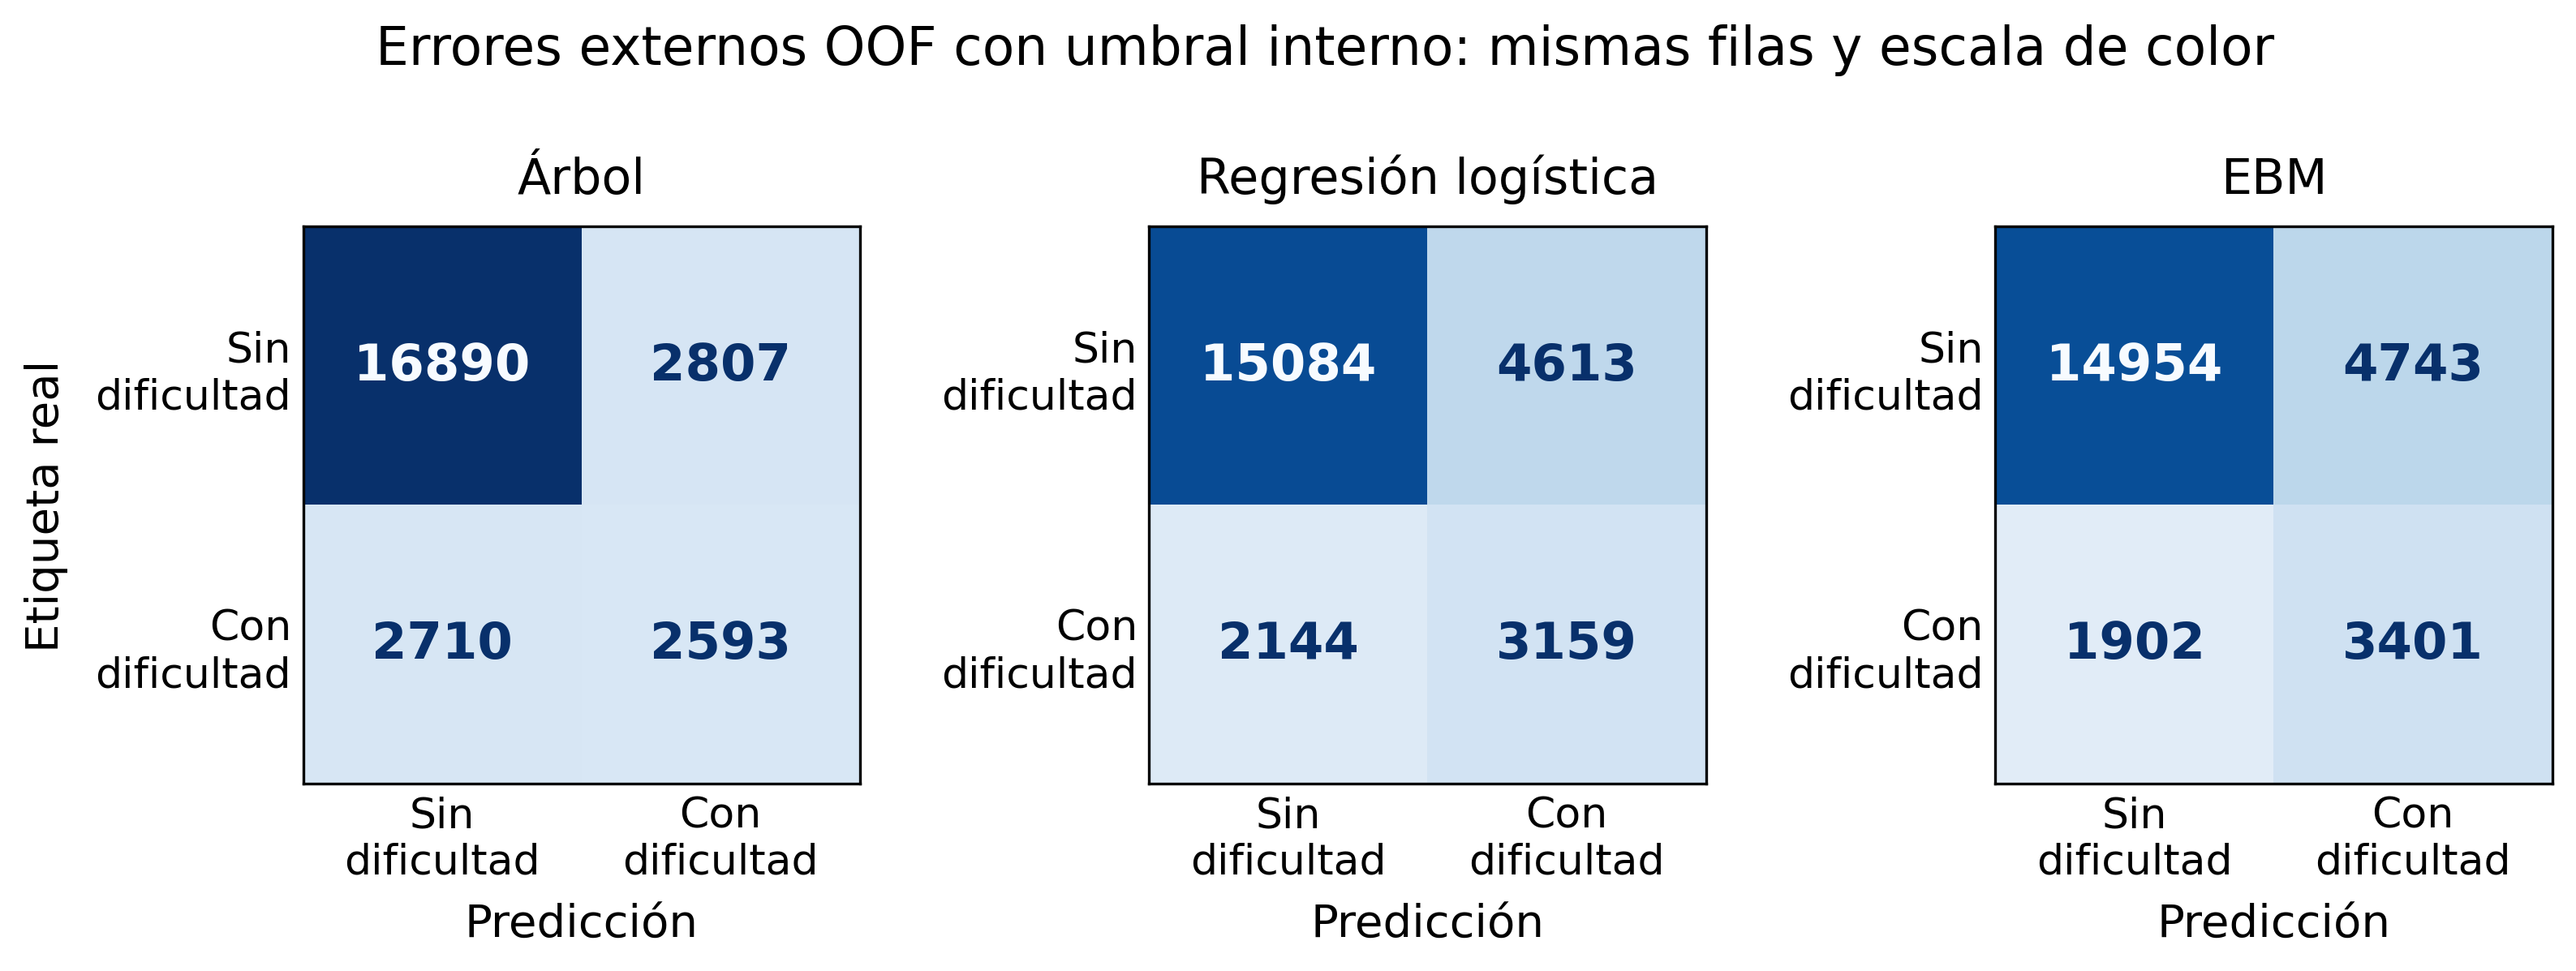
\includegraphics[width=\textwidth]{images/phase2_confusion_matrices.png}
	\caption{Matrices de confusión de los tres modelos con umbral interno. Filas: clase real; columnas: clase predicha; la escala de color es común a los tres paneles.}
	\label{fig:confusion}
\end{figure}

\section{Modelos}\label{sec:models}

Esta sección interpreta los modelos ajustados. Se distingue entre la estructura aprendida, es decir, reglas, coeficientes o funciones, y la evidencia de rendimiento ya presentada. La comparación se apoya en los mismos casos locales para mostrar qué explica cada familia y dónde coinciden o discrepan sus lecturas.

\subsection{Modelo lógico: reglas y probabilidades}

El árbol seleccionado puede leerse como una lista finita de reglas, la Figura~\ref{fig:tree} muestra su estructura. La configuración elegida en las cinco particiones externas fue profundidad máxima 3 y un mínimo de 500 registros por hoja, con umbral 0,25; el modelo resultante tiene profundidad efectiva 3, ocho hojas y quince nodos, y emplea tres variables.

\begin{figure}[H]
	\centering
	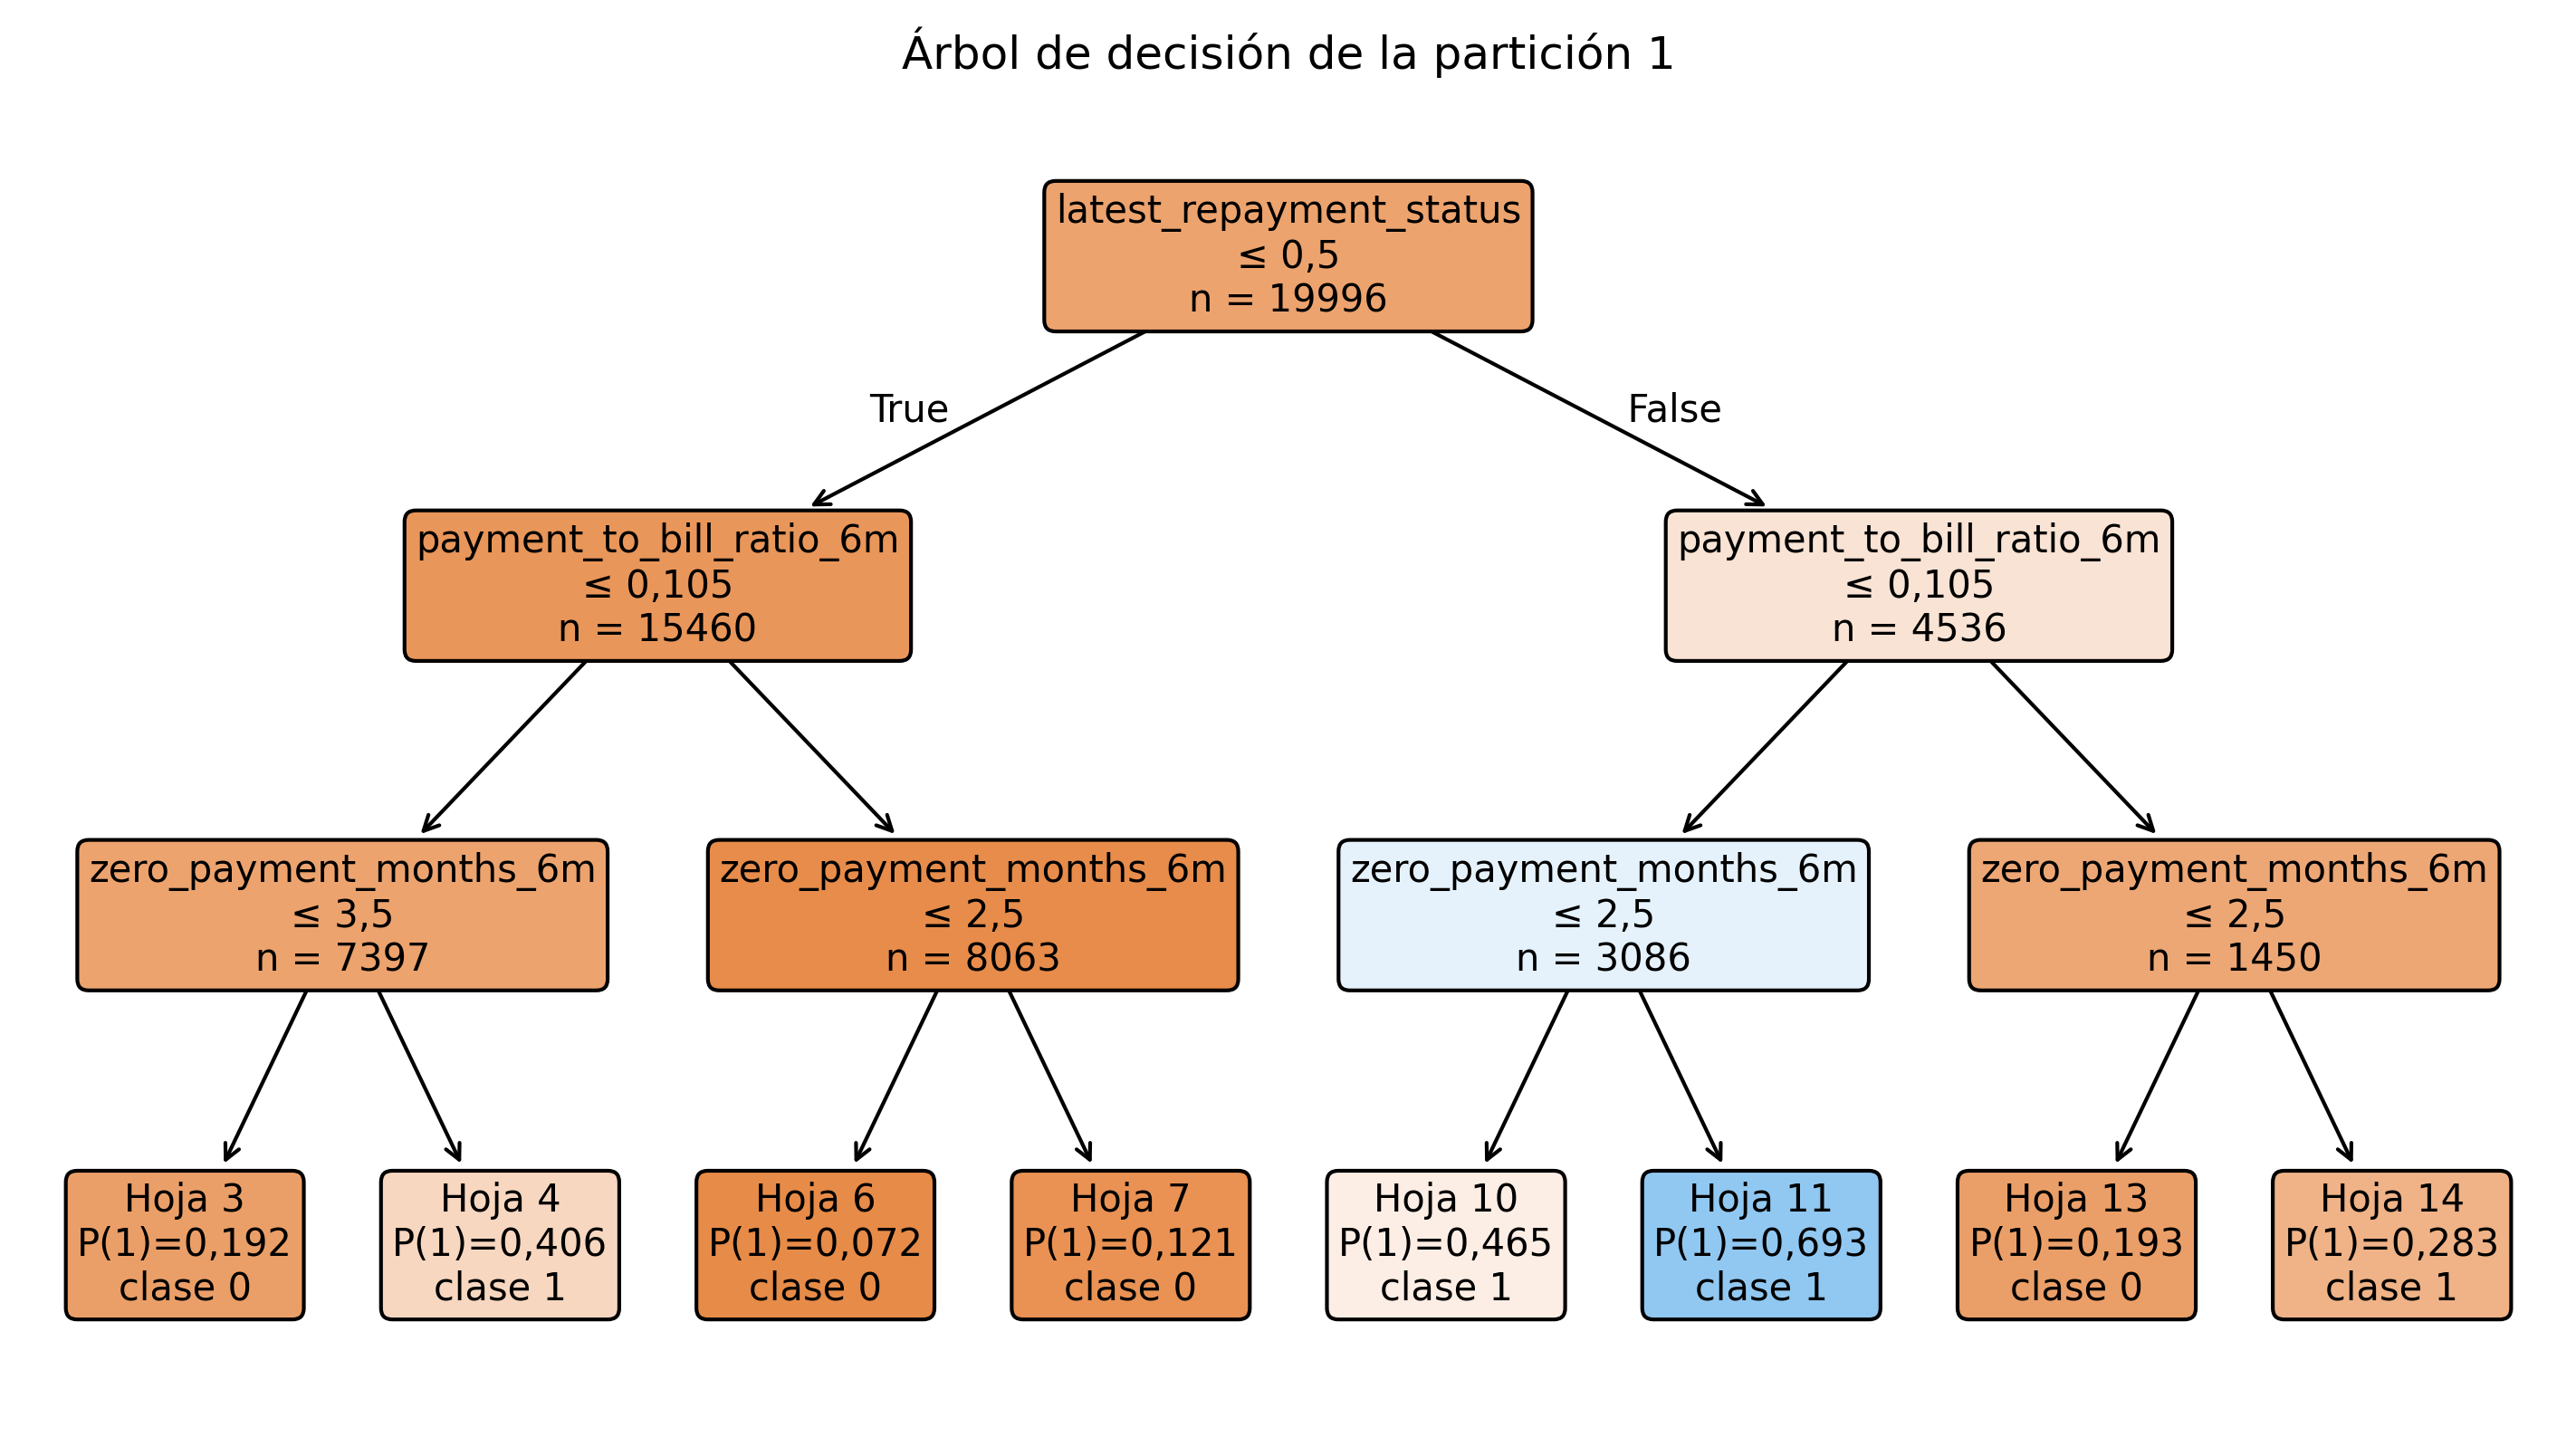
\includegraphics[width=\textwidth]{images/phase2_tree_names.png}
	\caption{Árbol de decisión de la partición 1. Cada nodo interno muestra la condición y el número de registros; cada hoja, la probabilidad estimada $P(1)$ y la clase asignada con el umbral 0,25.}
	\label{fig:tree}
\end{figure}

La raíz divide los registros según \var{latest_repayment_status}: $\le 0{,}5$ frente a $> 0{,}5$. El estado de pago más reciente es la primera distinción del modelo. La segunda división, repetida en ambas ramas, es \var{payment_to_bill_ratio_6m} $\le 0{,}105$, y el tercer nivel recurre a \var{zero_payment_months_6m} con umbrales $2{,}5$ o $3{,}5$. Las probabilidades de las hojas van de 0,0720 (hoja 6) a 0,6932 (hoja 11), de modo que el árbol no solo ordena los casos, sino que también expresa intensidades de riesgo muy distintas. La rama \var{latest_repayment_status} $\le 0{,}5$ contiene las hojas 3, 6 y 7, con probabilidades inferiores a 0,20, mientras que la hoja 4 alcanza 0,4062; la rama \var{latest_repayment_status} $> 0{,}5$ concentra tres de las cuatro hojas positivas (10, 11 y 14). Dentro de la rama de bajo \var{latest_repayment_status} y bajo \var{payment_to_bill_ratio_6m}, superar \var{zero_payment_months_6m} $= 3{,}5$ eleva la probabilidad de 0,1920 a 0,4062, más del doble. Con umbral 0,5 solo la hoja 11 predeciría la clase 1; al bajarlo a 0,25 se añaden las hojas 4, 10 y 14, la sensibilidad pasa del 14,31\,\% al 48,90\,\% y la precisión cae de 0,6812 a 0,4805. El comportamiento operativo del árbol depende, por tanto, de una decisión externa al ajuste.

La importancia Gini de la partición 1 es 57,25\,\% para \var{latest_repayment_status}, 29,71\,\% para \var{payment_to_bill_ratio_6m} y 13,05\,\% para \var{zero_payment_months_6m}; las otras doce variables no se usan. Esa concentración explica la legibilidad del modelo y también su límite, ya que tres variables resumen el riesgo y el resto de la información queda fuera. Las probabilidades de las hojas son frecuencias de entrenamiento, no probabilidades calibradas, es decir, que una hoja con 0,4646 se clasifique como positiva depende del umbral escogido (0,25 en nuestro caso).

La estructura se repite entre particiones, ya que los cinco árboles comparten la raíz \var{latest_repayment_status} $\le 0{,}5$ y la división \var{payment_to_bill_ratio_6m} $\le 0{,}105$ en ambas ramas. El tercer nivel es menos estable, con \var{zero_payment_months_6m} en cuatro modelos, \var{delayed_months_6m} en tres, \var{age} en dos, y \var{utilization_sep} y \var{credit_limit} en uno cada uno, con umbrales variables. La importancia media confirma ese patrón, con $0{,}5697 \pm 0{,}0066$ para \var{latest_repayment_status}, $0{,}3111 \pm 0{,}0232$ para \var{payment_to_bill_ratio_6m}, $0{,}0757 \pm 0{,}0531$ para \var{zero_payment_months_6m} y $0{,}0390 \pm 0{,}0358$ para \var{delayed_months_6m}. Cabe concluir que los dos primeros niveles son estables, mientras que las reglas terminales y sus probabilidades deben interpretarse con cautela.

\subsection{Coeficientes y odds ratios de la regresión logística}

La regresión logística supone que el logaritmo de las odds de dificultad de pago es una función lineal de los predictores transformados,
\[
\log\frac{P(Y=1\mid \mathbf{x})}{1-P(Y=1\mid \mathbf{x})}
= \beta_0 + \sum_{j=1}^{p}\beta_j z_j,
\]
donde $z_j$ representa una variable numérica estandarizada o una columna indicadora del one-hot. Cada $\beta_j$ cuantifica el cambio en log-odds asociado a una unidad de $z_j$ mientras el resto se mantiene fijo. Es una asociación condicional del modelo, no un efecto causal. La exponenciación da la odds ratio (OR), $\mathrm{OR}_j=e^{\beta_j}$, que expresa cuánto se multiplican las odds, no la probabilidad.

Las variables categóricas se codificaron con one-hot y la primera categoría como referencia, de modo que sus coeficientes se interpretan frente a ella. En la partición~1 las referencias son \var{female}, \var{graduate_school}, \var{married} y plan \var{no}. El término independiente, $-1{,}6022$, es el log-odds del perfil de referencia con todas las numéricas en su media, ya que están estandarizadas, y corresponde a una probabilidad de $16{,}77$\,\%. La tabla~\ref{tab:logistic-coefficients} recoge los ocho coeficientes principales de esa partición.

\begin{table}[H]
\centering
\footnotesize
\setlength{\tabcolsep}{6pt}
\begin{tabularx}{\textwidth}{@{}lrrX@{}}
\toprule
Entrada & Coeficiente & OR & Contraste \\
\midrule
\var{zero_payment_months_6m} & $0{,}5156$ & $1{,}6746$ & 1 DT $=1{,}7219$ meses \\
\var{repayment_assistance_plan_yes} & $0{,}4368$ & $1{,}5478$ & \var{yes} frente a \var{no} \\
\var{latest_repayment_status} & $0{,}4288$ & $1{,}5354$ & 1 DT  $=1{,}1215$ códigos \\
\var{utilization_sep} & $0{,}3841$ & $1{,}4683$ & 1 DT $=0{,}4050$ \\
\var{delayed_months_6m} & $0{,}2958$ & $1{,}3441$ & 1 DT $=1{,}5468$ meses \\
\var{total_payment_6m} & $-0{,}1682$ & $0{,}8500$ & 1 DT  $=58\,798{,}84$  \\
\var{maximum_repayment_delay_6m} & $-0{,}1216$ & $0{,}8900$ & 1 DT  $=1{,}0678$ meses\\
\var{sex_male} & $-0{,}0430$ & $0{,}9600$ & \var{male} frente a \var{female} \\
\bottomrule
\end{tabularx}
\caption{Coeficientes y odds ratios de la regresión logística en la partición~1. Las variables numéricas se expresan por una desviación típica (DT); las categóricas, frente a la categoría de referencia.}
\label{tab:logistic-coefficients}
\end{table}

Dos advertencias son necesarias para leer la tabla. Primero, los coeficientes de las numéricas se expresan por una desviación típica, no por una unidad original. Una OR de $1{,}6746$ en \var{zero_payment_months_6m} corresponde a $1{,}7219$ meses, y la de \var{utilization_sep}, $1{,}4683$, a $0{,}4050$ unidades de utilización. Segundo, una OR mayor que uno aumenta las odds, no la probabilidad, porque la conversión depende de la probabilidad de partida, de modo que multiplicar las odds por $1{,}5478$ no multiplica la probabilidad por esa cifra.

Los signos positivos principales corresponden a los meses sin pago, el plan de asistencia, el estado de devolución, la utilización y los meses con retraso, todos ellos se asocian con odds mayores. En sentido contrario, el total pagado, el retraso máximo y el sexo masculino presentan coeficientes negativos. El signo negativo del retraso máximo es condicional a los demás resúmenes de retraso, muy correlacionados entre sí; su correlación de Spearman con los meses con retraso es $0{,}982$. No implica que retrasarse proteja, sino que, una vez contabilizada la acumulación de meses, el máximo aporta información adicional en sentido opuesto. La lectura conjunta de variables correlacionadas exige cautela.

La penalización L1 fue seleccionada en las cinco particiones, con $C$ entre $0{,}1$ y $10$, y mantuvo entre 15 y 19 coeficientes no nulos de las 19 columnas transformadas. En la partición~1 anuló \var{education_other}, \var{education_unknown} y dos categorías de estado civil; un cero no prueba irrelevancia, pues depende de la penalización, de la colinealidad y de la frecuencia de la categoría. La estabilidad es razonable en los términos dominantes. El mismo conjunto de 19 entradas se repite en los cinco modelos, sin inversiones de signo, con magnitudes parecidas en los meses sin pago ($0{,}5051 \pm 0{,}0095$), el estado de devolución ($0{,}4151 \pm 0{,}0133$), la utilización ($0{,}3926 \pm 0{,}0120$) y el plan ($0{,}4520 \pm 0{,}0262$), mientras el total pagado se mantiene negativo ($-0{,}1692 \pm 0{,}0089$). Las categorías poco frecuentes alternan entre cero y no cero, por lo que su presencia concreta no debe interpretarse como un hallazgo estable. En conjunto, la logística ofrece una representación compacta y consistente en los términos dominantes, aunque su lectura exige recordar la escala estandarizada y la categoría de referencia.

\subsection{Funciones aditivas y formas aprendidas del EBM}

El EBM, ajustado sin interacciones, es un modelo aditivo generalizado en el que la puntuación de un registro se escribe como un valor independiente más la suma de quince funciones univariantes, una por predictor:
\[
\mathrm{logit}\, P(1 \mid \mathbf{x}) = \beta_0 + \sum_{j=1}^{15} f_j(x_j).
\]
En esta especificación, cada función depende de una sola variable y puede inspeccionarse por separado. La contribución $f_j(x_j)$ se expresa en log-odds, no una probabilidad ni un efecto causal, y solo se interpreta junto con las demás funciones. El valor independiente es $-1{,}6001$, de modo que un registro cuya suma de contribuciones sea cero tiene una probabilidad estimada del $16{,}80$ \%. Con quince funciones, el modelo es más expresivo que la regresión logística, pero sigue siendo aditivo y, por tanto, descomponible. Para un registro concreto, la predicción se reconstruye sumando el valor independiente y las quince contribuciones, lo que permite auditar por separado cada variable.

La tabla \ref{tab:ebm-importance} resume seis funciones seleccionadas de la partición 1. La importancia es la media del valor absoluto de la contribución y ordena las variables, pero no indica el signo ni la forma de la relación, que deben leerse en cada función. Una importancia alta puede combinar contribuciones de signo opuesto en distintos tramos, de ahí la necesidad de examinar la forma.

\begin{table}[H]
\centering
\small
\begin{tabularx}{\textwidth}{@{}l c X@{}}
\toprule
Variable & Importancia global & Lectura \\
\midrule
\var{payment_to_bill_ratio_6m} (R) & 0,3158 & Mayor peso; forma no monótona. \\
\var{latest_repayment_status} (S) & 0,2445 & Aumenta con los códigos de retraso, con mesetas. \\
\var{zero_payment_months_6m} (Z) & 0,2134 & Uno y dos meses, menor contribución que cero meses; desde tres, positiva. \\
\var{delayed_months_6m} & 0,1830 & Crece con la acumulación de retrasos. \\
\var{repayment_assistance_plan} & 0,1632 & \textit{yes} frente a \textit{no}: $+0{,}491$ log-odds. \\
\var{age} & 0,1349 & No lineal; extremos con menos respaldo. \\
\bottomrule
\end{tabularx}
\caption{Importancia global de seis funciones del EBM en la partición 1. La importancia es la media del valor absoluto de la contribución, en log-odds. La última columna resume la forma observada.}
\label{tab:ebm-importance}
\end{table}

La figura \ref{fig:ebm-shapes} muestra cuatro de estas funciones. El cociente pagos/facturas (R) es el de mayor importancia y el de forma menos regular. Su contribución es positiva en valores muy bajos, negativa en la región intermedia y de nuevo positiva en el extremo alto. Esa no monotonía sugiere que el cociente mezcla situaciones distintas; los valores altos pueden reflejar pagos extraordinarios o denominadores pequeños, por lo que no deben leerse como una señal unívoca de riesgo. El estado de pago reciente (S) y los meses con retraso \var{delayed_months_6m} aumentan en general con los códigos positivos y con la acumulación de retrasos, aunque presentan mesetas. En los meses sin pago (Z), uno y dos meses presentan una contribución menor que la de cero meses, mientras que desde tres la contribución es positiva y creciente. La edad sigue un patrón no lineal: mayor contribución en los jóvenes, negativa en parte de la edad adulta y creciente en el tramo superior, con menos respaldo en los extremos. La función del plan, que no aparece en la figura, asigna a \textit{yes} una contribución aproximadamente $0{,}491$ log-odds mayor que a \textit{no}.

\begin{figure}[H]
\centering
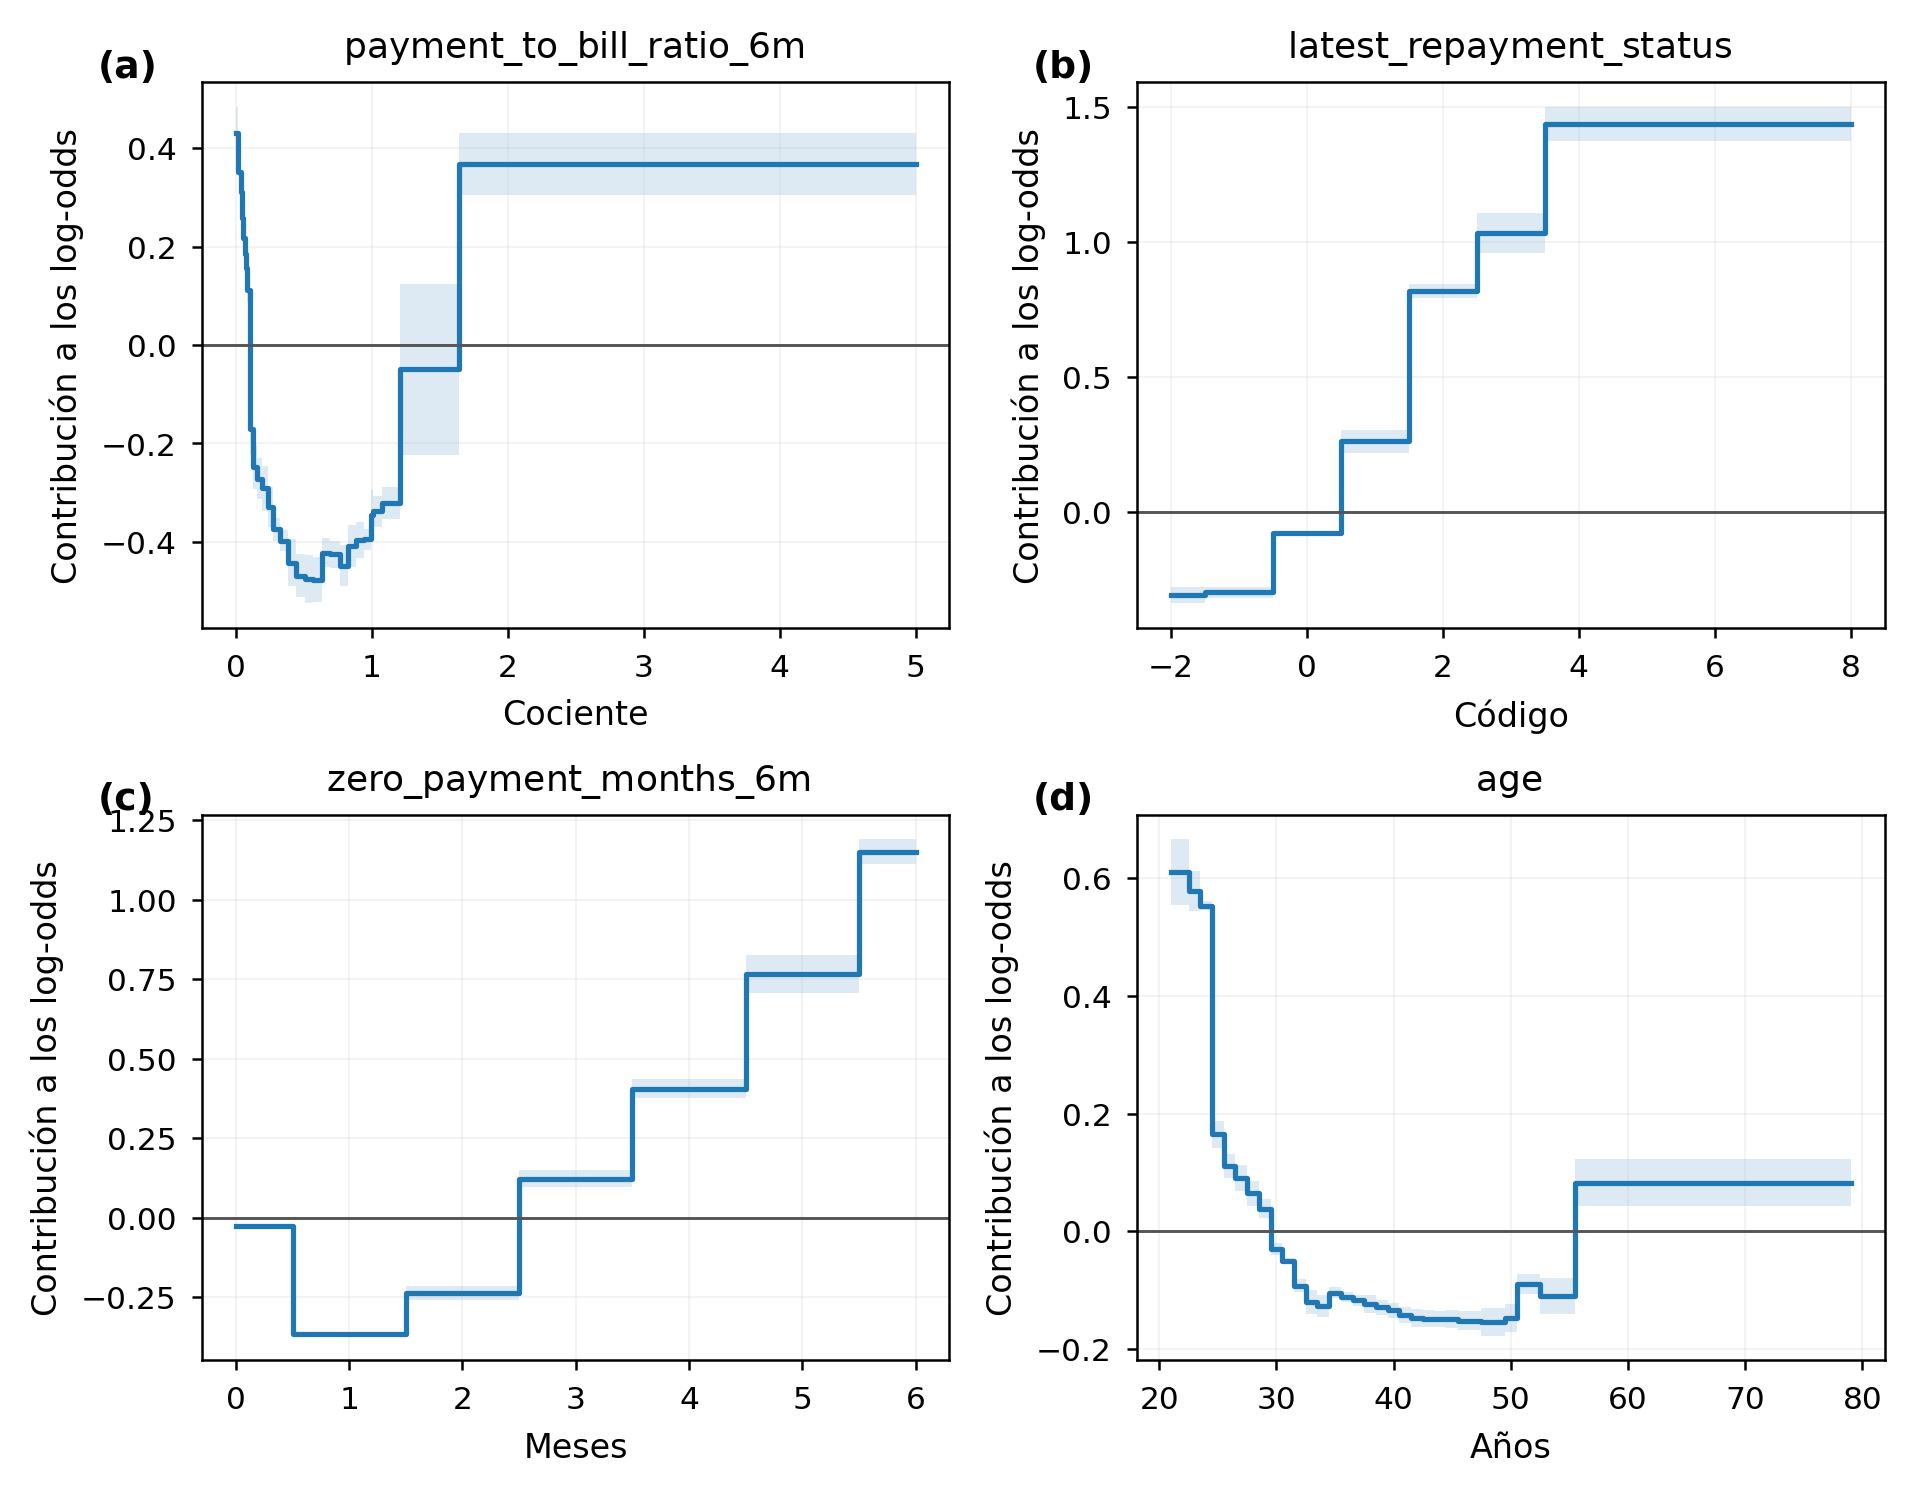
\includegraphics[width=0.7\textwidth]{images/phase2_ebm_shapes.png}
\caption{Cuatro funciones univariantes del EBM en la partición 1. En (a) se muestra el \var{payment_to_bill_ratio_6m}, en (b) el \var{latest_repayment_status}, en (c) \var{zero_payment_months_6m} y en (d) \var{age}. Las bandas representan la variabilidad entre las bolsas del modelo, no intervalos de confianza.}
\label{fig:ebm-shapes}
\end{figure}

En la figura \ref{fig:ebm-estability}, observamos que la estabilidad entre particiones es alta en lo esencial. R fue la función más importante en los cinco modelos, con una importancia media de $0{,}3072 \pm 0{,}0103$, después se repiten S, Z y \var{delayed_months_6m}, con cambios de orden. Las formas descritas reaparecen en las cinco particiones, la coincidencia de las formas es más informativa que el orden exacto de las importancias, y las discrepancias se concentran en los estados y recuentos altos y en las edades extremas, donde el respaldo de los datos es menor. En la partición 4 la contribución de S desciende del código 4 al 5, de modo que no puede afirmarse una monotonía universal. \var{maximum_repayment_delay_6m} presenta contribuciones positivas en algunos valores altos pese a su coeficiente logístico negativo. En conjunto, repetimos que estas formas son descripciones condicionales del modelo, no relaciones causales.


\begin{figure}[H]
	\centering
	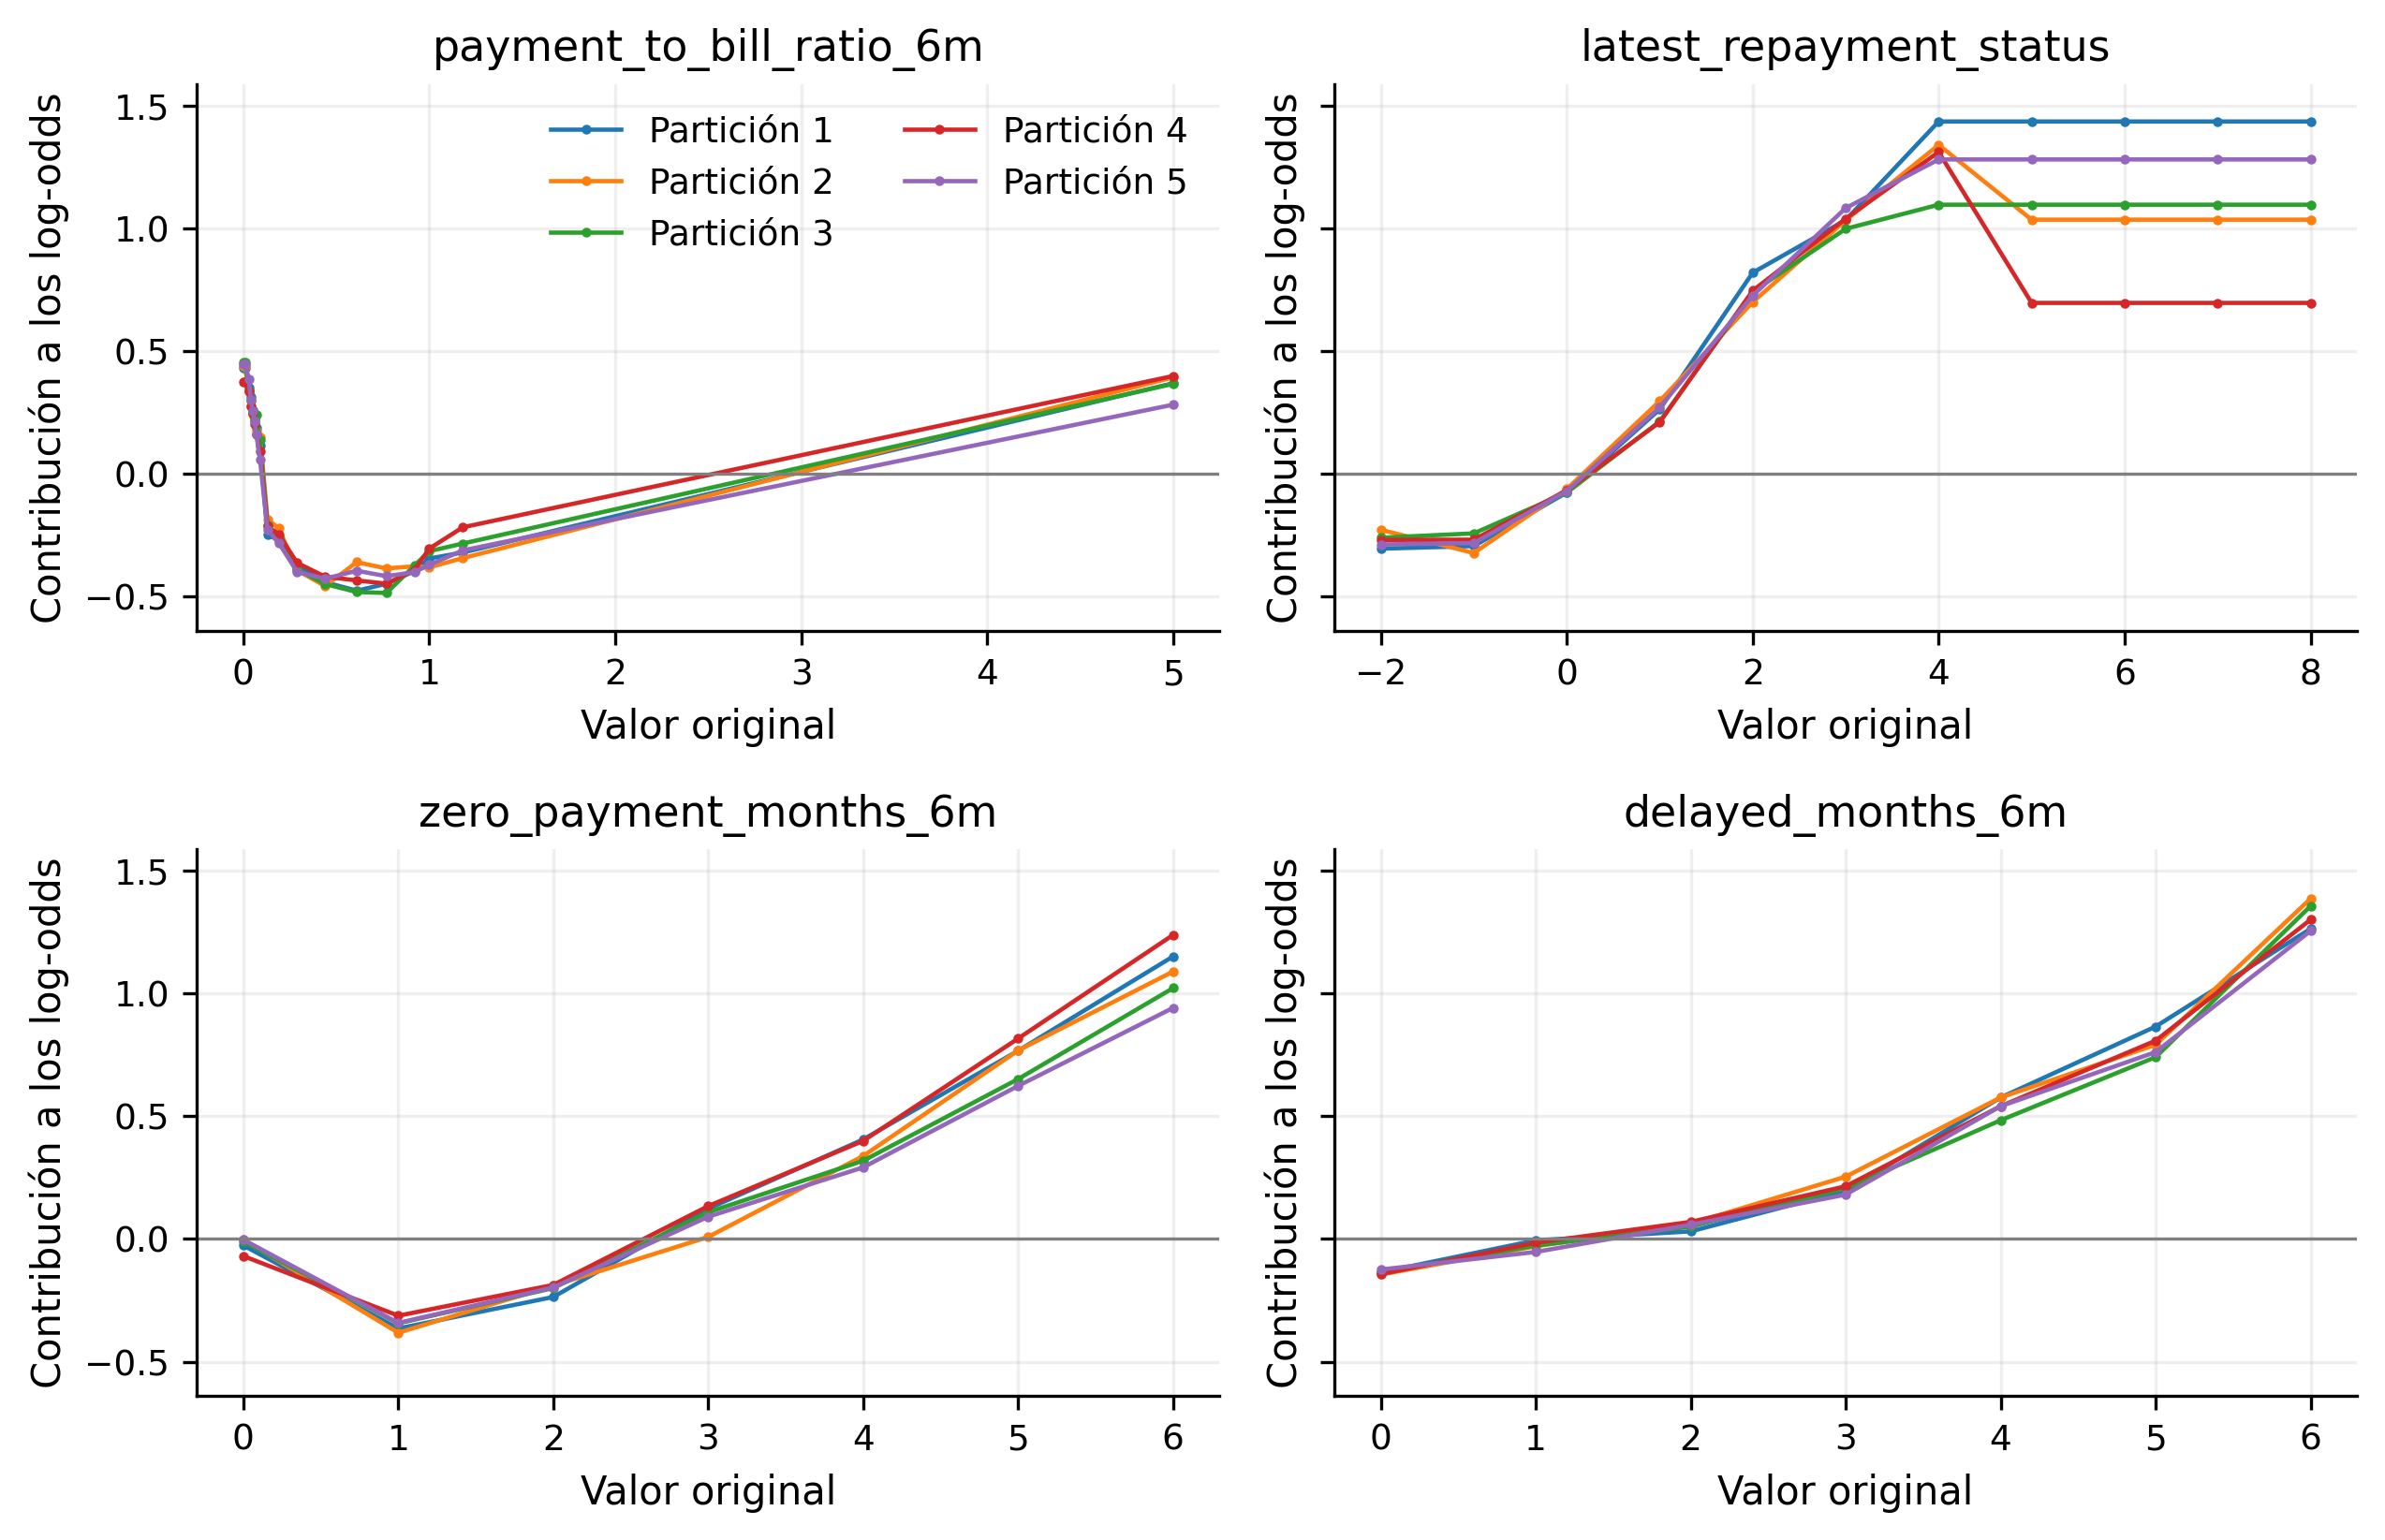
\includegraphics[width=0.7\textwidth]{images/phase2_ebm_stability.png}
	\caption{Estabilidad de cuatro funciones del EBM entre las cinco particiones. En (a) se muestra \var{payment_to_bill_ratio_6m}, en (b) \var{latest_repayment_status}, en (c) \var{zero_payment_months_6m} y en (d) \var{delayed_months_6m}. Cada color corresponde a una partición y la contribución se expresa en log-odds.}
	\label{fig:ebm-estability}
\end{figure}


\subsection{Explicaciones locales comparadas}

Para contrastar las explicaciones más allá de los resúmenes globales, se examinaron cuatro registros de la partición 1 con sus umbrales internos: $0{,}25$ para el árbol y la regresión logística, y $0{,}20$ para el EBM. La Tabla~\ref{tab:local-cases} recoge las probabilidades estimadas de la clase 1. Las cuatro probabilidades son inferiores a $0{,}5$, de modo que la decisión depende del umbral y no solo del orden entre modelos.


\begin{table}[H]
	\centering
	\small
	\caption{Cuatro casos locales de la partición 1 comparados entre familias. Los umbrales internos son $0{,}25$ para árbol y logística y $0{,}20$ para EBM. $P(1)$ denota la probabilidad estimada de la clase 1.}
	\label{tab:local-cases}
	\begin{tabularx}{\textwidth}{@{}c c X c c c@{}}
		\toprule
		Caso & Clase real & Escenario & Árbol $P(1)$ & Logística $P(1)$ & EBM $P(1)$ \\
		\midrule
		1 & $0$ & Acuerdo correcto, clase 0 & $0{,}0720$ & $0{,}0444$ & $0{,}0582$ \\
		2 & $1$ & Acuerdo correcto, clase 1 & $0{,}4646$ & $0{,}3997$ & $0{,}2663$ \\
		3 & $0$ & Árbol y logística aciertan; EBM falso positivo & $0{,}1920$ & $0{,}1832$ & $0{,}2110$ \\
		4 & $1$ & Falso negativo compartido & $0{,}1208$ & $0{,}1539$ & $0{,}1364$ \\
		\bottomrule
	\end{tabularx}
\end{table}

El caso 1 (clase 0) es un acuerdo correcto con explicaciones distintas. El árbol llega a la hoja 6 (\var{latest_repayment_status} $\le 0{,}5$, \var{payment_to_bill_ratio_6m} $> 0{,}105$, \var{zero_payment_months_6m} $\le 2{,}5$), la logística subraya \var{latest_repayment_status}, \var{zero_payment_months_6m} y \var{total_payment_6m} con contribuciones negativas, y el EBM destaca \var{payment_to_bill_ratio_6m} y \var{latest_repayment_status}. El único que aparece en las tres lecturas es \var{latest_repayment_status}, y el árbol comparte \var{zero_payment_months_6m} con la logística y \var{payment_to_bill_ratio_6m} con el EBM.

El caso 3 (clase 0) es el único desacuerdo. El árbol ($0{,}1920$) y la logística ($0{,}1832$) quedan por debajo de su umbral y aciertan, mientras que el EBM asigna $0{,}2110$, supera su umbral en $1{,}10$ puntos porcentuales y produce un falso positivo. Entre las atribuciones principales, cada par comparte una variable distinta (\var{zero_payment_months_6m} entre árbol y logística, \var{payment_to_bill_ratio_6m} entre árbol y EBM y \var{utilization_sep} entre logística y EBM) y ninguna coincide en los tres.

Los casos 2 y 4 no añaden un contraste nuevo. El 2 repite el acuerdo con \var{zero_payment_months_6m} aunque en sentidos opuestos ($+0{,}229$ en la logística y $-0{,}236$ en el EBM), y el 4 es un falso negativo compartido. Destacamos que las atribuciones son descripciones locales del modelo, es decir, coincidir en la decisión no implica coincidir en la explicación, y discrepar puede depender solo del umbral.

\section{Discusión}\label{sec:discussion}

\subsection{Rendimiento frente a interpretabilidad}

Los resultados ordenan las tres familias. El EBM obtiene la mejor discriminación (ROC-AUC $0{,}7755 \pm 0{,}0077$), seguido de la regresión logística ($0{,}7515 \pm 0{,}0075$) y del árbol ($0{,}7372 \pm 0{,}0044$). La ventaja del EBM se repite en exactitud equilibrada ($0{,}6997$) y F1 ($0{,}5068$), mientras que el árbol conserva la mayor exactitud ($0{,}7793$) y la mayor precisión ($0{,}4805$). Esa combinación no designa un ganador absoluto. Si el uso previsto es priorizar un número reducido de revisiones con pocos falsos positivos, el árbol resulta defendible; si el objetivo es no dejar casos sin detectar, el EBM ofrece una sensibilidad notablemente mayor ($0{,}6405$ frente a $0{,}4890$ del árbol y $0{,}5955$ de la logística). La diferencia no puede atribuirse solo a la expresividad, ya que también cuentan la forma funcional del modelo, la penalización y el presupuesto de búsqueda.

La interpretabilidad tampoco es una sola dimensión. El árbol de referencia de la partición 1 se lee de un vistazo, con ocho reglas, tres variables y una jerarquía aplicable manualmente; entre las cinco particiones se utilizan de tres a cinco variables. Esa brevedad tiene un precio, porque solo una parte de los quince predictores participa en cada ajuste, las probabilidades son frecuencias de entrenamiento y la decisión cambia de forma abrupta con el umbral. La logística es compacta (quince a diecinueve coeficientes no nulos), pero exige manejar log-odds, categorías de referencia y contrastes por desviación típica; su lectura es más lenta que la del árbol aunque su forma sea global y aditiva. El EBM es el más expresivo, con quince funciones, cada una con su escala y su forma, algunas no monótonas. Inspeccionarlas cuesta más, pero permite ver dónde y con qué signo actúa cada variable, algo que el árbol solo insinúa. En suma, el árbol gana en acceso inmediato, la logística en compacidad y el EBM en fidelidad descriptiva; la elección depende de quién audite el modelo.

Con umbral $0{,}5$ los tres modelos superan la exactitud mayoritaria del $78{,}79$\,\%, pero detectan menos del $30$\,\% de los positivos. Con el umbral interno la sensibilidad sube entre 34,23 y 35,14 puntos porcentuales y la exactitud cae por debajo de esa referencia. No hay umbral universal sin costes, porque fijarlo decide qué fallo se tolera, no es una propiedad del modelo.

\subsection{De ocho a seis reglas}

Con umbral $0{,}25$, las hojas 6 y 7 del árbol predicen ambas clase 0 y las hojas 10 y 11 ambas clase 1. Fusionarlas produce dos reglas con probabilidades $0{,}0800$ y $0{,}5353$, de modo que el árbol puede presentarse como una lista de seis reglas con las mismas decisiones. El ahorro es real pero modesto, y se paga con probabilidades más gruesas, ya que se pierde la diferencia entre $0{,}0720$ y $0{,}1208$, y entre $0{,}4646$ y $0{,}6932$. Los otros dos desdoblamientos no pueden eliminarse sin perder las hojas positivas 4 y 14. Con umbral $0{,}5$ la lista podría ser aún más corta, pero la sensibilidad descendería, de modo que existe un compromiso entre simplicidad y rendimiento. Si el destino del modelo es una lista de comprobación, seis reglas son preferibles; si es la priorización fina de casos, conviene conservar las ocho.

\subsection{Mejoras y límites}

Las mejoras posibles se agrupan en tres frentes. En el árbol, la poda por coste-complejidad comentada, que nos permite crecer un árbol grande y recortar ramas con una penalización por hoja elegida por validación, podría sustituir la rejilla por un criterio sistemático. En la logística, los splines o las interacciones entre variables darían margen a efectos hoy forzados a ser lineales, a costa de perder la lectura de un coeficiente por variable. En el EBM, imponer monotonía en variables como los retrasos podría alinear las formas con el dominio y facilitaría su lectura.


Los límites son claros. Las cinco particiones proceden de entrenamientos solapados y no son réplicas independientes, de modo que su dispersión mide simplemente la sensibilidad al reparto. La familia se eligió con los mismos resultados que se comparan, lo que puede introducir optimismo; la exactitud equilibrada interna de $0{,}7007$ usada para seleccionar el umbral final no acredita una mejora externa sobre el $0{,}6997$ de la comparación. El test sin etiquetas no permite una comprobación independiente del rendimiento del modelo final; además, el carácter semisintético del ejercicio limita su extrapolación a una población real.

\section{Conclusión}\label{sec:conclusion}

El proyecto se propuso predecir la dificultad de pago del mes siguiente con modelos que, además de discriminar, explicaran sus decisiones. Se compararon un árbol, una regresión logística y un EBM sobre las mismas cinco particiones externas agrupadas, con validación anidada, selección por ROC-AUC y umbral por exactitud equilibrada. Esa homogeneidad permite comparar las familias sin que el reparto las favorezca.

El EBM obtuvo la mayor ROC-AUC ($0{,}7755 \pm 0{,}0077$) y la mejor exactitud equilibrada ($0{,}6997$ con umbral interno), seguido de la logística ($0{,}7515$) y del árbol ($0{,}7372$). La ventaja del EBM se repite en las cinco particiones, aunque el árbol conserva la mayor exactitud ($0{,}7793$) y precisión ($0{,}4805$). El umbral interno eleva la sensibilidad en más de $34$ puntos porcentuales, a costa de precisión y de exactitud, que cae por debajo de la referencia mayoritaria. No hay umbral neutro, porque fijarlo equivale a elegir qué error se tolera.

El modelo final fue un EBM sin interacciones, con \var{max_bins}=32, $10$ observaciones mínimas por hoja y umbral $0{,}20$. Aplicado al test, asigna $3\,208$ casos a la clase 0 y $1\,792$ a la clase 1, y se guarda en \texttt{outputs/test.csv} conservando filas y valores originales; sin etiquetas no pueden calcularse métricas.

La interpretabilidad no es una sola propiedad. Las reglas del árbol son inmediatas pero gruesas, los coeficientes de la logística compactos pero con referencias y escalas, y las funciones del EBM más fieles pero más costosas de inspeccionar. Una misma decisión no implica la misma explicación, y el umbral forma parte de ella.

Los límites acotan las conclusiones. Las cinco particiones proceden de entrenamientos solapados, no de réplicas independientes, así que su dispersión mide la sensibilidad al reparto. La familia se eligió con los resultados que se comparan, lo que puede introducir optimismo: el $0{,}7007$ final no acredita mejora externa sobre el $0{,}6997$. El test sin etiquetas impide afirmar generalización real, y la ventaja del EBM también depende de factores como la forma funcional o la penalización. Las mejoras posibles son la poda por coste-complejidad en el árbol, los splines o interacciones en la logística y la monotonía en variables como los retrasos en el EBM como se comentaba en la sección anterior.

El valor del proyecto reside en combinar rendimiento y explicaciones fieles sin confundir asociación con causa.

\section{Referencias}\label{sec:references}

\nocite{statement,dictionary,xai}
\printbibliography[heading=none]

\section{Uso de la inteligencia artificial generativa}\label{sec:ai}

Durante el desarrollo del proyecto se utilizó Codex (OpenAI) como apoyo para organizar y revisar el notebook, proponer código y visualizaciones, y revisar la redacción. Para este informe se empleó un asistente de IA generativa en la organización y la edición del texto, así como para detectar inconsistencias y mejorar la claridad. El grupo ejecutó el código, verificó las cifras y asume la responsabilidad del contenido. Las decisiones de diseño, selección de modelos e interpretación de los resultados correspondieron al grupo.


\end{document}
